\documentclass[a4paper,12pt]{article}
\usepackage[utf8]{inputenc}

\usepackage[utf8]{inputenc}
\usepackage[spanish]{babel}
\usepackage{amsmath}
\usepackage{amsfonts}
\usepackage{amssymb}
\usepackage{float}
\usepackage{graphicx}
\usepackage[left=2cm,right=2cm,top=2cm,bottom=2cm]{geometry}
\usepackage{fancyhdr}
\pagestyle{fancy}
\usepackage{hyperref}
\usepackage[usenames,dvipsnames]{color}
\hypersetup{colorlinks=true}
\hypersetup{colorlinks, citecolor=BurntOrange, linkcolor=BurntOrange, urlcolor=Blue}
\usepackage{url}
\usepackage{listings}
\usepackage{courier}
\lstset{language=ada}

%opening
\rhead{Estructura de Dades}
\title{\Huge{Estructura de Dades}\\\vspace{1cm} \Huge{\textbf{Pràctica de l'Assignatura}}}
\author{Pablo Riutort, Alfredo Ucendo}

\begin{document}

\maketitle
\pagebreak
\tableofcontents
\pagebreak

\lstset{basicstyle=\footnotesize\ttfamily,breaklines=true}
\lstset{framextopmargin=50pt,frame=bottomline}

\section{t\_frequencies.ads}

\begin{lstlisting}
with arbre_caracters; use arbre_caracters;

package t_frequencies is

type abecedari is private;

-- rang de valors dels indexos de les taules

procedure tbuida (tfreq: out abecedari);
procedure omplir (tfreq: out abecedari; fname: in String; ok: out boolean);
procedure mostra (tfreq: in abecedari);

no_rang : exception;
mal_us :exception;


type iterator is private;

procedure primer(ce: in abecedari; it: out iterator);
procedure succesor(ce: in abecedari; it: in out iterator);
procedure consulta(ce: in abecedari; it: in iterator; k: out Rang_Valors; x: out Float);
function esValid(it: in iterator) return boolean;
 --~ 
pragma inline(primer,succesor,consulta,esValid);


private 

	Maxim : constant Integer := 200;

	-- tipus per recordar quins caracters apareixen
	type T_Caracters is array (Rang_Valors) of Character; 
	
	-- tipus per comptar el nombre d'aparicions de cada caracter
	type T_Frequencies is array (Rang_Valors) of Integer; 


	-- declaracio de la 'taula de freqüencies' per treballar
	type abecedari is 
		record 
			Caracters   : T_Caracters;  
			Frequencies : T_Frequencies;  
			Limit       : Integer;    -- nombre d'elements incorporats a les taules. 
                                      -- Tambe indica el lloc on es troba el darrer
                                      -- element incorporat.
		end record; 

	--iterador
	type iterator is
		record
			k: Rang_Valors;
			valid: boolean;
		end record;
   
end t_frequencies;

\end{lstlisting}

\section{t\_frequencies.adb}
\begin{lstlisting}
 with Ada.Text_Io; use Ada.Text_Io;
with Ada.Float_Text_io; use Ada.Float_Text_io;

package body t_frequencies is 

	Origen : File_Type;  -- fitxer d'origen
	Nom_Fitxer_Aparicio  : constant String := "frequencies.txt";
	Lletra : Character;  -- Variable per llegir el contingut del fitxer origen
	
	procedure tbuida (tfreq: out abecedari) is
	begin
		for Index in Rang_Valors'Range loop
			tfreq.Frequencies:=(others=>0);
		end loop;
		tfreq.Limit := 0;
	end tbuida;
   
	procedure omplir (tfreq: out abecedari; fname: in String; ok: out boolean) is separate;
   
	-- Procediment per guardar el resultat de la feina feta
	procedure mostra (tfreq: in abecedari) is separate;
	
	--Iteradors
	procedure primer (ce: in abecedari; it: out iterator) is
		k: Rang_Valors renames it.k;
		e: T_Frequencies renames ce.Frequencies;
	begin
		k:=Rang_Valors'First;
		while not (e(k) > 0) and k<Rang_Valors'Last loop
			k:=Rang_Valors'succ(k);
		end loop;
		it.valid:= (e(k)>0);
	end primer;	
	
	
	procedure succesor(ce:in abecedari; it: in out iterator) is
		k: Rang_Valors renames it.k;
		e: T_Frequencies renames ce.Frequencies;
	begin
		if not it.valid then raise mal_us; end if;
		if k < Rang_Valors'last then
			k:=Rang_Valors'succ(k);
			while not (e(k) > 0) and k<Rang_Valors'Last loop
				k:=Rang_Valors'succ(k);
			end loop;
			it.valid:= (e(k)>0);
		else
			it.valid:=false;
		end if;
	end succesor;
	
	function esValid(it: in iterator) return boolean is
	begin
		return it.valid;
	end esValid;
	
	procedure consulta(ce: in abecedari; it: in iterator; k: out Rang_Valors; x: out Float) is
		c: T_Frequencies renames ce.Frequencies;
		valid: boolean renames it.valid;
		freq: Integer;
	begin
		if not valid then raise mal_us; end if;
		k:= it.k; 
		freq:=c(k);
		x:=float(freq*100)/float(ce.Limit);
	end consulta;
	
end t_frequencies;

\end{lstlisting}

\subsection{t\_frequencies-omplir.adb}
\begin{lstlisting}
 separate (t_frequencies)

procedure omplir (tfreq: out abecedari; fname: in String; ok: out boolean) is
begin
	--Control de excepciones
	begin 
		-- Obrir el fitxer origen per llegir
		Open(Origen, In_File, fname);
	exception 
		when Name_Error => ok := False; 
	end; 
	

	-- Recorregut fins al final del fitxer.
	-- End_Of_File ens indica si hi ha o no qualque cosa per llegir.
	while not End_Of_File(Origen) loop

			Get(Origen, Lletra);			
			if Lletra'Valid then
				tfreq.Frequencies(Lletra):=tfreq.Frequencies(Lletra) + 1;
				tfreq.Limit:= tfreq.Limit + 1;
			else
				raise no_rang;
			end if;

	end loop;
	
	-- Tancar el fitxer
	Close (Origen);
	-- Fer saber que s'ha acabat
	Put_Line("Taula de freqüències generada.");
   
end omplir;

\end{lstlisting}
\pagebreak
\subsection{t\_frequencies-mostra.adb}
\begin{lstlisting}
 separate (t_frequencies)

procedure mostra (tfreq: in abecedari) is
   Fitxer : File_Type;
   pct: Float;
begin
   Create(Fitxer, Out_File, Nom_Fitxer_Aparicio);
   
	for Index in Rang_Valors'Range loop
		if tfreq.Frequencies(Index)/=0 then
			pct:=float(tfreq.Frequencies(Index)*100)/float(tfreq.Limit); -- càlcul del % d'aparacions
			Put(Fitxer, Index'Img & " ->" & tfreq.Frequencies(Index)'Img);
			Put(Fitxer," (");Put(Fitxer,pct,FORE=>1, AFT=>2, EXP=>0);Put_Line(Fitxer,"%)");
		end if;
	end loop;
	
   Close(Fitxer);
   put_line("Taula de freqüències guardada a '" & Nom_Fitxer_Aparicio & "'");
   
end mostra;

\end{lstlisting}


\section{arbre\_b.ads}
\begin{lstlisting}
 generic 

type item is private;
with procedure Put_Item(x:in item);

package arbre_b is
type arbre is private;
type tipusdenode is (n_fulla, n_pare);
type pnode is private;

procedure buit(t:out arbre);
procedure construeix (t:out arbre; lt,rt:in arbre; f: out float);
procedure construeix (t:out arbre; x:in item; f: in float);
procedure arrel (t:in arbre; tnd:out tipusdenode);
procedure esquerra (t:in arbre; lt:out arbre);
procedure dreta (t:in arbre; rt:out arbre);
procedure get (t:in arbre; x: out item);
function es_buit (t:in arbre) return boolean;
--las dos siguientes pendientes de implementar
function "<" (x1,x2: in arbre) return boolean;
function ">" (x1,x2: in arbre) return boolean;

--procediments auxiliars
procedure mostra(t:in arbre);

mal_us: exception;
overflow: exception;

--private specification
private

	type node;
	type pnode is access node;
	
	type node (tnd:tipusdenode) is record
		case tnd is
			when n_pare =>  fe: pnode;
							fd: pnode;
			when n_fulla => x: item;
		end case;
	end record;
	
	type arbre is 
		record
			root:pnode;
			f:float;
	end record;
	
end arbre_b;
	

\end{lstlisting}


\section{arbre\_b.adb}
\begin{lstlisting}
 with Ada.Text_Io; use Ada.Text_Io;
with Ada.Float_Text_io; use Ada.Float_Text_io;

package body arbre_b is

--crea un arbre buit
procedure buit (t:out arbre)is
	p: pnode renames t.root;
begin
	p:=null;
end buit;

--fa un node interior
procedure construeix (t:out arbre; lt,rt:in arbre; f: out float)is
	p: pnode renames t.root;
begin
	p:= new node(n_pare);
	p.fe:=lt.root;
	p.fd:=rt.root;
	--sumamos las probabilidades.
	f:=lt.f+rt.f;
	t.f:=f;
exception
	when storage_error => raise overflow;
end construeix;

--fa un node fulla
procedure construeix (t:out arbre; x:in item; f: in float)is
	p: pnode renames t.root;
begin
	--declaracion del nodo hoja
	p:= new node(n_fulla);
	p.x:=x;
	--construccion del arbol
	t.f:=f;
exception
	when storage_error => raise overflow;
end construeix;

procedure arrel (t:in arbre; tnd:out tipusdenode)is
	p: pnode renames t.root;
begin
	 tnd:=p.tnd;
exception
	when constraint_error => raise mal_us;
end arrel;

--fa fill esquerr el segon paràmetre del primer paràmetre
procedure esquerra (t:in arbre; lt:out arbre) is
	p: pnode renames t.root;
	pe: pnode renames lt.root;
begin
	pe:=p.fe;
exception
	when constraint_error => raise mal_us;
end esquerra;

--fa fill dret el segon paràmetre del primer paràmetre
procedure dreta (t:in arbre; rt:out arbre)is
	p: pnode renames t.root;
	pd: pnode renames rt.root;
begin
	pd:=p.fd;
exception
	when constraint_error => raise mal_us;
end dreta;


--funcions de major, menor i buit--

function es_buit (t:in arbre) return boolean is
	p: pnode renames t.root;
begin
	return p=null;
end es_buit;

function "<" (x1,x2: in arbre) return boolean is
	f1:float renames x1.f;
	f2:float renames x2.f;
begin
	return (f1 < f2);
end "<";

function ">" (x1,x2: in arbre) return boolean is
	f1:float renames x1.f;
	f2:float renames x2.f;
begin
	return (f1 > f2);
end ">";

procedure get (t: in arbre; x:out item) is
	begin
		x:=t.root.x;
end get;

--PROCEDIMENTS AUXILIARS

--funcio auxiliar per imprimir un node
procedure mostra (pn: in pnode;d: in Integer) is 
	tipus: tipusdenode renames pn.tnd;
	--~ nivell: constant Integer:=d+1;	--actualitza el nivell de profunditat
	root_simbol: constant character:= '*';
	shift: constant string:= "  "; 
begin	
	if (pn /= null) then --si està buit no fa res
		for i in 1..d loop put(shift);	end loop;
		case tipus is
			when n_pare =>  
				put("└──> ");				
				put(root_simbol);new_line;				
				mostra(pn.fe,d+1);new_line;
				mostra(pn.fd,d+1);
			when n_fulla => 
				put("└──> ");
				Put_Item(pn.x);
		end case;
	end if;
end mostra;

--saca el arbol a un fichero de texto
procedure mostra (t:in arbre) is
   --campos del arbol
   r: pnode renames t.root;
   f: float renames t.f;
   d: constant Integer:=0;   --profunditat de s'arbre
begin
	new_line;
    Put("[");Put(f,FORE=>1, AFT=>2, EXP=>0);Put("%]");
	new_line;
	mostra(r,d);
	new_line(2);
end mostra;
end arbre_b;

\end{lstlisting}


\section{d\_heap.ads}
\begin{lstlisting}
 generic
	
	size: positive := 200; --heuristica?
	type item is private;
	with function "<" (x1,x2: in item) return boolean;
	with function ">" (x1,x2: in item) return boolean;

package d_heap is

	type heap is limited private;
	
	bad_use: exception;
	space_overflow: exception;
	
	procedure buit   	(q: out heap);
	function es_buit 	(q: in heap) return boolean;	
	procedure posa		(q: in out heap; x: in item);
	procedure elimina_darrer(q: in out heap);
	function darrer		(q: in heap) return item;

	private
	
		type mem_space is array (1..size) of item;
		
		type heap is
			record
				a: mem_space;
				n: natural;
			end record;

end d_heap;

\end{lstlisting}


\section{d\_heap.adb}
\begin{lstlisting}
 with Ada.Integer_Text_IO; use Ada.Integer_Text_IO;
with Ada.Text_IO;use Ada.Text_IO;

package body d_heap is

--crea un monticle buit
procedure buit (q:out heap)is
	n: natural renames q.n;
begin
	n:=0;
end buit;

--miram si es buit
function es_buit (q:in heap) return boolean is
	n: natural renames q.n;
begin
	return n=0;
end es_buit;

--posa un element al monticle
procedure posa (q:in out heap; x:in item) is
	a: mem_space renames q.a;
	n: natural renames q.n;
	i: natural;	--index a un node del monticle
	pi: natural; --index al pare del node
begin

	n:=n+1; --augmentam el nombre d'elements de la coa
	i:=n; --l'index del node que visitam a la coa
	pi:=n/2; --index del pare del node que visitam a la coa
	
	--mentres hi hagi un pare per a aquest element, llavors miram si l'element a ficar es menor que el del seu pare,
	--en cas afirmatiu, vol dir que s'ha de recolocar a la coa de prioritats.
	while pi>0 and then a(pi)>x loop
		a(i):=a(pi);
		i:=pi;
		pi:=i/2;
	end loop;
	--si no tenim un node major que el del propi objecte, hem acabat
	a(i):=x;
end posa;

--elimina el darrer element de l'arbre
procedure elimina_darrer(q: in out heap)is
	a: mem_space renames q.a;
	n: natural renames q.n;
	i: natural;
	ci: natural; --index per al darrer fill de i
	x: item; --item auxiliar.
begin
	--si el monticle està buit
	if n=0 then raise bad_use; end if;
	x:=a(n); --guardam el darrer element de la coa
	
	--pasam al calcular com quedarà el darrer dins el nostre monticle
	n:=n-1; --decrementam els elements de la coa
	i:=1; --posa el node al primer element de la coa
	ci:=i*2; --calculam el fill del node anterior
	
	if ci<n and then a(ci+1)<a(ci) then ci:=ci+1; end if;
	
	--mentres quedin fills i el nostre element sigui menor que l'element darrer
	while ci<=n and then a(ci)<x loop
		--feim actualitzacio de tal manera que podem recorrer l'arbre cap a baix
		a(i):=a(ci);
		i:=ci;
		ci:=i*2;
	end loop;
	--si l'element darrer es major que l'actual, hem acabat
	a(i):=x;
end elimina_darrer;

--retorna el darrer element de la coa
function darrer (q:in heap) return item is
	a: mem_space renames q.a;
	n: natural renames q.n;
begin
	if n=0 then raise bad_use; end if; --la coa està buida!
	return a(1); --el "darrer element" de la coa es troba al principi.
end darrer;

end d_heap;

\end{lstlisting}


\section{arbre\_caracters.ads}
\begin{lstlisting}
 with arbre_b;
with Ada.Text_IO;

package arbre_caracters is
	
	subtype Rang_Valors is Character Range Character'First..Character'Last;
	package a_c is new arbre_b (item => Rang_Valors, Put_Item => Ada.Text_IO.Put);

end arbre_caracters;

\end{lstlisting}
\pagebreak

\section{codifica.ads}
\begin{lstlisting}
 with t_frequencies; use t_frequencies;
with arbre_caracters; use arbre_caracters, arbre_caracters.a_c;
with Direct_IO,Sequential_IO;

package codifica_f is

	type Entrada is record
		Lletra: Character;
		Codi: string(1..257);
	end record;
	
	package Dir_IO is new Direct_IO(Entrada);use Dir_IO;
	package Seq_IO is new Sequential_IO(character);use Seq_IO;
	
	procedure genera_codis(Taula: in abecedari; a: out arbre; fname: in string);
	procedure codifica(fname_text,fname_codis: in string);	
	procedure postordre(a: in arbre; fname: in String);	
	procedure recorregut(a: in arbre; file: in Dir_IO.File_Type;registre: in out Entrada;d: in integer);

end codifica_f;

\end{lstlisting}


\section{codifica.adb}
\begin{lstlisting}
 with d_heap;
with Ada.Text_IO; use Ada.Text_IO;
with Ada.Characters.Latin_1; use Ada.Characters.Latin_1;
with Ada.Strings.Fixed;use Ada.Strings.Fixed;
with Ada.Strings.Unbounded;use Ada.Strings.Unbounded; 

package body codifica_f is
procedure genera_codis(Taula: in abecedari; a: out arbre; fname: in string) is

package tree_heap is new d_heap (item => arbre,"<" => "<",">" => ">");	use tree_heap;

arbre_consulta,arrel,fe,fd: arbre; 
f: float; 
it: iterator;
k: arbre_caracters.Rang_Valors; 		--caracter del nostre conjunt 
monticle: heap; 						--monticle on guardarem els arbres
final: boolean:= false;
f_codis: constant String:= fname&".co";

begin
	buit(monticle);		--construim un monticle buit
	primer(Taula, it);	--es situa al primer element(iterador)
	-- construeix un arbre per cada caràcter i l'afegeix al monticle
	while (esValid(it)) loop
		consulta(Taula, it, k, f);
		construeix(arbre_consulta,k,f);
		posa(monticle,arbre_consulta);
		succesor(Taula, it);
	end loop;
	
	-- agrupa els arbres del monticle fins obtenirne un amb tots el caràcters
	while not final loop	
		fe:= darrer(monticle);
		elimina_darrer(monticle);
		if not es_buit(monticle) then
			fd:= darrer(monticle);
			elimina_darrer(monticle);
		end if;
		final:=es_buit(monticle); 		--condicio final, tenim l'arbre complet al heap
		construeix(arrel,fe,fd,f);
		posa(monticle,arrel);
	end loop;
	a:=darrer(monticle);
	postordre(a,f_codis);				-- calcula taula de codificacio de l'arbre obtingut
	
end genera_codis;

procedure postordre(a: in arbre; fname: in String) is
	Fitxer: Dir_IO.File_Type;
	registre: Entrada;
	begin
		Put_line("----------------------------------------");
		Put_line("      Simbol"&HT&"|      Codi");
		Put_line("----------------------------------------");
		Create(Fitxer, Out_File,fname);
		recorregut(a, Fitxer,registre,0);
		Close(Fitxer);
		Put_line("----------------------------------------");
		put_line("Taula de codificacio generada i guardada a '" & fname & "'");
end postordre;
		
procedure recorregut(a: in arbre; file: in Dir_IO.File_Type; registre: in out Entrada;d: in integer) is
	lt, rt: arbre;
	tnd: tipusdenode; 					-- discriminant
	codi_e,codi_d: Unbounded_String; 	-- codis dels fills
	reg_fe,reg_fd: Entrada; 			-- registres succesors
	begin
		-- obtenim el codi 'base' per als fills
		codi_e:= to_unbounded_string(registre.codi(1..d));
		codi_d:=codi_e;		
		arrel(a,tnd);
		if (tnd = n_pare) then
			-- cap a l'esquerra
			esquerra(a,lt);							
			Append(codi_e,"0");											-- afegim el codi del successor
			Move(to_string(codi_e),reg_fe.Codi);						-- guardam el codi complet al registre
			recorregut(lt, file,reg_fe,d+1);		
			-- cap a la dreta
			dreta(a,rt);
			Append(codi_d,"1");
			Move(to_string(codi_d),reg_fd.Codi);
			recorregut(rt, file,reg_fd,d+1);
		else
			get(a,registre.Lletra);										--llegim el caracter actual y el guardam al registre
			Write(file,registre,Rang_Valors'Pos(registre.Lletra)); 		-- escribim el registre al fitxer(posicio = valor ASCII)
			Put_line(HT&registre.Lletra&""&HT&"|"&HT&registre.codi);
		end if;
end recorregut;

procedure codifica(fname_text,fname_codis: in string) is
text: Seq_IO.File_Type;
codis: Dir_IO.File_Type;
resultat: Ada.Text_IO.File_Type;
Lletra: Rang_Valors; 																	--lletra que llegim del fitxer de text
registre: Entrada;																		--codi que llegim de la taula de codis
fname_resultat: constant string :="c_"&fname_text;
begin
	Open(text,In_File,fname_text);
	Open(codis,In_File,fname_codis);
	Create(resultat,Out_File,fname_resultat);
	put_line("Text codificat(guardat a '"& fname_resultat &"'):");
	while not End_Of_File(text) loop
			Read(text, Lletra);															-- llegim el caràcter
			if (Lletra'Valid) and then (Rang_Valors'Pos(Lletra) <= Size(codis)) then			
				Set_Index(codis,Rang_Valors'Pos(Lletra));								-- apuntam al codi corresponent
				Read(codis,registre);
				if (registre.Lletra /= Lletra) then									-- aquesta lletra no te codi
					put(Lletra);
					put(resultat, lletra);
				else 																	-- te codi
					for i in 1..registre.codi'length loop
						exit when (registre.codi(i) = ' ');
						put(registre.codi(i));
						put(resultat, registre.codi(i));	
					end loop;
										
				end if;
			else
				put(Lletra);
				put(resultat, lletra);
			end if;
	end loop;
	Close(resultat);
	Close(text);
	Close(codis);
end codifica;
		
end codifica_f;

\end{lstlisting}


\section{decodifica.ads}
\begin{lstlisting}
 with arbre_caracters; use arbre_caracters, arbre_caracters.a_c;
with Sequential_IO;

package decodifica_f is
	
	fname_ne: constant string:= "nombre_estats.n";
	Significat_especial: constant Rang_valors:= Rang_valors'First; --null char
	type simbol_t is new integer range 0..1;
	type Transicio is record
		Estat_inicial: integer;
		simbol: simbol_t;
		Estat_final: integer;
		Significat: Rang_valors;
	end record;
	
	transicio_error: exception;
	recorregut_error: exception;

	package Seq_IO is new Sequential_IO(Transicio);use Seq_IO;
	package Int_IO is new Sequential_IO(Integer);use Int_IO;
		
	type automata is			
      record
         Simbol_0: Integer;
         Simbol_1: Integer;
         Caracter: Rang_Valors;
      end record;

	type t_automata is array (Integer range <>) of automata; --el array de automatas contiene la tabla, el indice del array seran los estados inciales
	
	procedure decodifica(f_text,f_recurs: in string);
	procedure genera_transicions(a: in arbre;fname: in string);	
	procedure recorregut(a: in arbre; file: in Seq_IO.File_Type; Estat: in out integer);
	procedure genera_transicio(file: in Seq_IO.File_Type; Estat_inicial: in integer; simbol: in simbol_t;Estat_final: in integer;significat: in Rang_valors);
    function NFA (file: in Seq_IO.File_Type;estats: in integer) return t_automata;
    procedure mostra_automata(a: in t_automata);
    
    private 
    
    function nombre_estats return integer;

end decodifica_f;

\end{lstlisting}


\section{decodifica.adb}
\begin{lstlisting}
 with Ada.Text_IO; use Ada.Text_IO;
with Ada.Characters.Latin_1; use Ada.Characters.Latin_1;
with Ada.IO_exceptions;

package body decodifica_f is
procedure genera_transicions(a: in arbre;fname: in String) is
	Fitxer: Seq_IO.File_Type;
	estats: Int_IO.File_Type;				--fitxer on guardam el nombre d'estats
	Estat: integer:=1;
	f_transicions: constant String:=fname&".de";
	begin
		Create(Fitxer, Out_File,f_transicions);
		recorregut(a, Fitxer,Estat);
		Close(Fitxer);
		new_line;put_line("Taula de transicions generada i guardada a '" & f_transicions & "'");
		Create(estats,Out_File,fname_ne);
		Write(estats,Estat); 		-- guardam el nombre de estats
		Close(estats);
		put_line("Nombre d'estats guardat a '" & fname_ne);		
end genera_transicions;

procedure recorregut(a: in arbre; file: in Seq_IO.File_Type; Estat: in out integer) is
	tnd: tipusdenode; 					-- discrimina
	lt, rt: arbre;
	lletra: Character;
	estat_local: integer;
begin
	arrel(a,tnd);
	estat_local:=Estat;
	if (tnd = n_pare) then
		Estat:=Estat+1;
		esquerra(a,lt);
		genera_transicio(file,estat_local,0,Estat,Significat_especial);						
		recorregut(lt, file,Estat);
		
		Estat:=Estat+1;
		dreta(a,rt);
		genera_transicio(file,estat_local,1,Estat,Significat_especial);	
		recorregut(rt, file,Estat);
	else
		get(a,lletra);
		genera_transicio(file,estat_local,0,0,lletra);
	end if;
end recorregut;

procedure genera_transicio(file: in Seq_IO.File_Type; Estat_inicial: in integer; simbol: in simbol_t;Estat_final: in integer;significat: in Rang_valors) is
	registre: Transicio;
begin
	--~ new_line;put(Estat_inicial'img&" "&simbol'img&" "&Estat_final'img&" "&significat);
	registre:=(Estat_inicial,simbol,Estat_final,significat);
	write(file,registre);
end genera_transicio;

function NFA (file: in Seq_IO.File_Type;estats: in integer) return t_automata is
t: Transicio;
t_a: t_automata(1..estats);
begin
	--lectura del fichero dado por parametro
	while not End_Of_File (file) loop
		read(file,t);
		--~ new_line;put(t.Estat_inicial'img&" "&t.simbol'img&" "&t.Estat_final'img&" "&t.significat);
		if (t.simbol = 0)then
			t_a(t.Estat_inicial).Simbol_0:=t.Estat_final;
			if (t.significat /= significat_especial) then t_a(t.Estat_inicial).Simbol_1:=0; end if;
		else
			t_a(t.Estat_inicial).Simbol_1:=t.Estat_final; 
		end if;
		t_a(t.Estat_inicial).Caracter:=t.Significat;
	end loop;	
	mostra_automata(t_a);
	return t_a;
end NFA;

procedure mostra_automata(a: in t_automata) is
begin
	new_line;
	Put(HT&"Estat"&HT&"|"&HT&"0"&HT&"|"&HT&"1"&HT&"|  Caràcter"&HT&"");new_line;
	Put("-----------------------------------------------------------------");new_line;
	for i in a'Range loop
		Put(HT & i'Img & HT & "|");
		Put(HT & a(i).simbol_0'Img & HT & "|");
		Put(HT & a(i).simbol_1'Img & HT & "|");
		Put(HT & a(i).Caracter);
		new_line;
	end loop;
end mostra_automata;

procedure decodifica(f_text,f_recurs: in string) is
	transicions: Seq_IO.File_Type;			-- taula de transicions
	text: Ada.Text_IO.File_Type;			-- text a decodificar
	resultat: Ada.Text_IO.File_Type;		-- resultat de la decodificacio
	fname_res: constant string:= "d_"&f_text;
	ne: integer;
	lletra: character;
	Estat,Estat_final: integer;
	t_a: t_automata(1..nombre_estats);
begin	
		ne:= nombre_estats;			--llegim el nombre d'estats
		put_line("Llegim la taula de transicions del fitxer '"&f_recurs&"':");
		--carregam la taula de transicions
		Open(transicions, In_File, f_recurs);
		t_a:=NFA(transicions,ne);
		Close(transicions);
		
		put_line("Inici decodificacio del fitxer '"&f_text&"'");
		--carregam la taula de transicions
		Open(text, In_File, f_text);
		Create(resultat, Out_File, fname_res);
		Get(text,lletra);
		while not End_Of_File(text) loop
			if (lletra = '1' or else lletra = '0') then			-- es un codi
				Estat:=1;
				-- cercam sa lletra
				while not End_Of_File(text) and then (Estat /= 0) loop
					if (lletra = '1') then
						Estat_final:= t_a(Estat).simbol_1;
					else -- lletra = '0'
						Estat_final:= t_a(Estat).simbol_0;
					end if;
					if (Estat_final = 0) then
						put(t_a(Estat).Caracter);		-- hem trobat el caràcter
						put(resultat,t_a(Estat).Caracter);
						Estat:=0;						-- marcam el final						
					else
						Estat:=Estat_final;				-- actualitzam s'estat
						get(text,lletra);						
					end if;
				end loop;
			else 										-- es una lletra
				put(lletra);
				put(resultat,lletra);
				Get(text,lletra);
			end if;
		end loop;
		Close(resultat);
		Close(text);
		put_line("Resultat de la decodificacio guardat a '"&fname_res&"'.");
exception
		when ada.io_exceptions.end_error => Close(resultat);Close(text);
end decodifica;

function nombre_estats return integer is
f_estats: Int_IO.File_Type;
ne: integer;
begin
	Open(f_estats, In_File, fname_ne);
	read(f_estats,ne);
	Close(f_estats);
return ne;
end nombre_estats;
end decodifica_f;

\end{lstlisting}


\section{cryptomatic.adb (Main)}
\begin{lstlisting}
 with Ada.Command_line; use Ada.Command_Line;
with t_frequencies; use t_frequencies;
with Ada.Text_IO; use Ada.Text_IO;
with codifica_f,decodifica_f; use codifica_f,decodifica_f;
with arbre_caracters; use arbre_caracters,arbre_caracters.a_c;
 
procedure cryptomatic is
	a : arbre;
	Taula: abecedari;
	ok: boolean;
begin   
   
   if (Argument_Count /= 3) then 
		Put_line("Nombre de paràmetres incorrecte, haurien de ser 3");
   else		
		if (Argument(1) = "c") then			-- codifica			
			codifica(Argument(2),Argument(3));	
		else 
			if (Argument(1) = "d") then 		-- decodifica
				decodifica(Argument(2),Argument(3));
			else 
				if (Argument(1) = "r") then		-- genera els recursos .co i .de
					-- Arg 2: nom del fitxer a partir del qual generam el recursos
					-- Arg 3: nom que donam als recursos (ex: "re" -> re.co / re.de)
					tbuida(Taula);      
					omplir(Taula, Argument(2), ok);		-- genera una taula d'aparicions de caracters donat un fitxer
					mostra(Taula); 						-- Guarda el nombre d'aparicions de cada caracter
					genera_codis(Taula,a,Argument(3));	-- Genera una taula de codis per a cada caracter (*.co)
					mostra(a);							-- imprimeix s'arbre resultant	
					genera_transicions(a,Argument(3));
				else
					Put_line("Ordre no reconeguda, nomes 'c','d' o 'r'");
				end if;
			end if;
		end if;
   end if;
end cryptomatic;

\end{lstlisting}
\pagebreak

\section{Altres}

\subsection{Limpia}
A aquesta pràctica ha estat inclòs l'arxiu 'limpia' que es un script que fa:
\begin{center}
  \begin{lstlisting}
  rm -f *.ali *.o *.swp *~
  rm *.co *.de
  \end{lstlisting}
\end{center}
Amb això aconseguim eliminar arxius transitoris i de proves per a poder fer feina més còmodament

\subsection{git}
Per a l'elaboració d'aquesta pràctica s'ha emprat git, podeu trobar el repositori de la pràctica a \url{https://github.com/pabloriutort/Estructura-de-dades.git}.

\pagebreak
\section{Joc de proves}
Ús del cryptomatic: ./cryptomatic comanda, arxiu1, arxiu 2.\\\
\newline
Comanda:
\begin{itemize}
 \item \textbf{r}: Genera una taula de codis a partir de l'arxiu1 amb el nom arxiu2 més l'extensió '.co' (arxiu2.co) i també un arxiu2 amb l'extensió '.de' amb la taula de transicions.
 \item \textbf{c}: Codifica l'arxiu1 amb un arxiu2 amb extensió '.co'.
 \item \textbf{d}: Decodifica l'arxiu1 amb un arxiu2 amb extensió '.de'.
\end{itemize}

A continuació adjuntam el joc de proves que s'ha fet:

\subsection{prueba 1: Generar el arxius (.co) i (.de) a partir d'un fitxer de text}

\begin{lstlisting}
./cryptomatic r lorem.txt recurs

lorem.txt:
\end{lstlisting}

Lorem ipsum ad his scripta blandit partiendo, eum fastidii accumsan euripidis in, eum liber hendrerit an.\\\

\begin{lstlisting}
Resultats:
\end{lstlisting}

\begin{itemize}
 \item guarda la taula de freqüències generada al fitxer 'frequencies.txt'.
 \item un arxiu anomenat 'recurs.co' amb la taula de codificació.
 \item un arxiu anomenat 'recurs.de' amb la taula de transicions.
 \item imprimeix per pantalla la taula de codificació.
 \item imprimeix per pantalla l'arbre obtingut
 \item Output per consola:
\end{itemize}

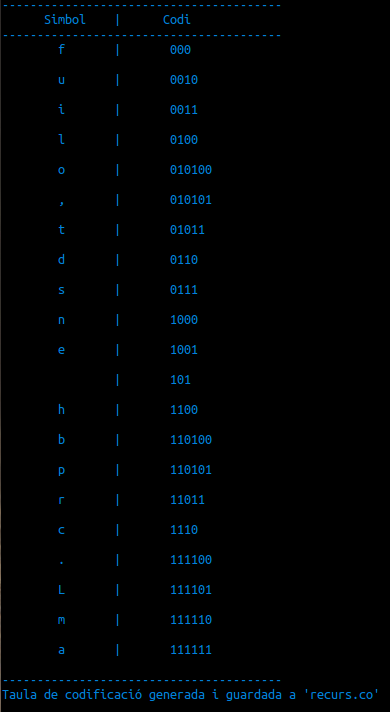
\includegraphics{tabla.png}

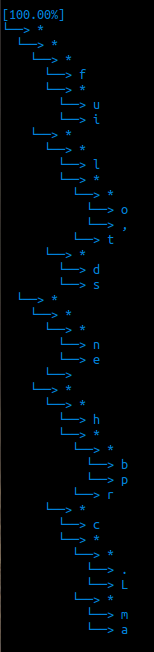
\includegraphics{arbol.png}

\begin{lstlisting}
Taula de transicions generada i guardada a 'recurs.de'
Nombre d'estats guardat a 'nombre\_estats.n'
\end{lstlisting}
\pagebreak
\subsection{prueba 2: Codificar un text}

\begin{lstlisting}
./cryptomatic c segismundo.txt recurs.co 

segismundo.txt:
\end{lstlisting}
Yo sueño que estoy aquí destas prisiones cargado, y soñé que en otro estado más lisonjero me vi. ¿Qué es la vida? Un frenesí. ¿Qué es la vida? Una ilusión, una sombra, una ficción, y el mayor bien es pequeño, que toda la vida es sueño, y los sueños, sueños son.
\begin{lstlisting}
Resultats:
\end{lstlisting}

- mostra per pantalla el resultat de la codificació y també el guarda al fitxer 'c\_segismundo.txt'

\begin{lstlisting}
c\_segismundo.txt:
-----------------

Y010100101011100101001ñ010100101q001010011011001011101011010100y101111111q0010í1010110100101110101111111101111011101011
1011001101110011010100100010010111101111011111111011g1111110110010100010101101y1010111010100ñé101q001010011011001100010
1010100010111101101010010110010111010111111110110010100101111110á01111010100001101110101001000j100111011010100101111110
1001101v0011111100101¿Q0010é101100101111010100111111101v00110110111111?101U1000101000110111001100010010111í11110010¿Q0010é101100101111010100111111101v00110110111111?101U100011111110100110100001001110011ó100001010110100101000111111101011101010011111011010011011111111010101101001010001
111111010000011111011100011ó1000010101101y10110010100101111110111111y01010011011101110100001110011000101100101111011101
011001q00101001ñ010100010101101q001010011010101101010001101111111010100111111101v00110110111111101100101111010111001010
01ñ010100010101101y10101000101000111101011100101001ñ0101000111010101101011100101001ñ010100011110101110101001000111100
\end{lstlisting}


\subsection{prueba 3: Decodificar un text}

\begin{lstlisting}
./cryptomatic d c\_segismundo.txt recurs.de

c\_segismundo.txt:
-----------------

Y010100101011100101001ñ010100101q001010011011001011101011010100y101111111q0010í1010110100101110101111111101111011101011
1011001101110011010100100010010111101111011111111011g1111110110010100010101101y1010111010100ñé101q001010011011001100010
1010100010111101101010010110010111010111111110110010100101111110á01111010100001101110101001000j100111011010100101111110
1001101v0011111100101¿Q0010é101100101111010100111111101v00110110111111?101U1000101000110111001100010010111í11110010¿Q0010é101100101111010100111111101v00110110111111?101U100011111110100110100001001110011ó100001010110100101000111111101011101010011111011010011011111111010101101001010001
111111010000011111011100011ó1000010101101y10110010100101111110111111y01010011011101110100001110011000101100101111011101
011001q00101001ñ010100010101101q001010011010101101010001101111111010100111111101v00110110111111101100101111010111001010
01ñ010100010101101y10101000101000111101011100101001ñ0101000111010101101011100101001ñ010100011110101110101001000111100

Resultats:

\end{lstlisting}
- imprimeix la taula de transicions que s'ha fet servir per inicialitzar l'automata.
- mostra per pantalla el resultat de la decodificació y també el guarda al fitxer 'd\_c\_segismundo.txt'

\begin{lstlisting}
d\_c\_segismundo:
\end{lstlisting}
Yo sueño que estoy aquí destas prisiones cargado, y soñé que en otro estado más lisonjero me vi. ¿Qué es la vida? Un frenesí. ¿Qué es la vida? Una ilusión, una sombra, una ficción, y el mayor bien es pequeño, que toda la vida es sueño, y los sueños, sueños son.

\end{document}
